%%%%%%%%%%%%%%%%%%%%%%%%%%%%%%%%%%%%%%%%%%%%%%%%%%%%%%%%%%%%%%%%%%%%%%%%%
%
% Time
%
%%%%%%%%%%%%%%%%%%%%%%%%%%%%%%%%%%%%%%%%%%%%%%%%%%%%%%%%%%%%%%%%%%%%%%%%%
\subsection{\label{subsec:time-in-databases}Time in Databases}
The concept of time has been studied in databases for a long time. A true standard for adding temporal aspects to relational databases does not exist, but there is a consensus in the literature \cite{Dyreson1994} on what is called a \emph{temporal database}: a temporal database is a database dealing with some aspects of time in its schema.
In a temporal DBMS, a \textbf{chronon} is the shortest duration of time supported by the system. In temporal databases, some temporal attributes can be managed without treating the attribute differently from non-temporal attributes. The time described by such an attribute is called \textbf{user defined time} (\emph{UDT}). In addition to UDT, the following types of time can be discerned in a temporal database, all of which are handled exceptionally by the DBMS:

\begin{itemize}
	\item
	\textbf{Transaction time} (\emph{TT}) \cite{Rowe1987,Jensen1991} denotes the time when the fact (object) is stored in the database. It is usually append-only: as the past cannot be changed, TT cannot be changed either. Furthermore, at the moment of insertion, a TT can be neither in the past nor in the future.
	\item
	\textbf{Valid time} (\emph{VT}) \cite{Jensen1994,Sarda1990,McKenzie1981} denotes the time when the fact (object) is true in the modelled reality. A fuzzy extension has been proposed by \cite{Garrido2009}. 
%	\item
%	User defined time: It is an uninterpreted attribute. The domain is date/time. The query language has no special support for it.
	\item
	\textbf{Decision time} (\emph{DT}) \cite{Nascimento1995,Chakravarthy1994,Etzion1992,Ozsoyoglu1995} denotes the time when an event was decided to happen. 
	\end{itemize}
	
	E.g., consider a database containing employee contract descriptions. The time when the employee's contract is valid, represented by an interval, is VT. The time when the employee's contract is stored in the database is the TT. The time when the decision for hiring this employee was made is the DT.

% is a non-decomposable unit of time.  it  There are two ways to represent a chronon: as a point or as an interval \cite{655777}.

When working with these time concepts, the Data Manipulation Language (\emph{DML}, which is part of the standard database querying language SQL) is extended to deal with possible temporal inconsistencies within the data and to handle more complex (temporal) queries. 
%Next to these concepts, also \textbf{user defined time} (\emph{UDT}) is discerned. UDT is an uninterpreted attribute in the date/time domain. This means that the attribute uses the date/time domain, but the database model does not treat the attribute differently from non-temporal attributes.
Depending on the time managed, a database is classified as either a \textbf{Valid Time Database} (\emph{VTDB}), a \textbf{Transaction Time Database} (\emph{TTDB}), a \textbf{bi-temporal database} (both valid and transaction time are managed) or a \textbf{tri-temporal} or \emph{multitemporal} database (valid time, transaction time and decision time are managed).

%\subsection{Temporal Elements}
%%	
%	In order to define a temporal database model, some basic elements should be defined \cite{Dyreson:1994:CGT:181550.181560}:
%	\begin{itemize}
%	\item A	\textbf{chronon} is a non-decomposable unit of time. In a temporal DBMS, it is the shortest duration of time supported by the system. There are two ways to represent a chronon: as a point or as an interval \cite{655777}.
%	\item
%	\emph{Event}: An instant of time. Usually, an event is said to be occur during time $t$ if it occurs during the chronon represented by $t$.
%	\item
%	\emph{Interval}: The time between two events. The representation is very often a set of contiguous chronons.
	%\item
	%\emph{Span}: A directed duration of time. A duration is an amount of time with known  lenght but no specific starting or ending chronons. The span can be either positive, denoting a forward motion of time or negative, denoting a backward motion of time.
%	\item A	\textbf{timestamp} is a time value associated with some object in the database.	
	
%	\item The	\textbf{lifespan} (of a database object)is the time over which it is defined. The lifespan of a valid time object denotes the time when the corresponding object exists. The lifespan of a transaction time object is the value of the timestamp.
	
	
	
	
	
%	Depending on the type of time the meaning is different:
%		\begin{itemize}
%		\item
%		Lifespan of a valid time object: Refers the time when the corresponding object exists.	
%		\item
%		Lifespan of a transaction time object: The transaction time of a database object refers when the object is stored in the database. The lifespan is the value of the timestamp.		
%		\end{itemize}
%	\end{itemize}
	
%	In the temporal database thesaurus, \emph{'Snapshot'} is the word for non-temporal matters. As a temporal database is a generalization for relational databases, an \emph{snapshot database} is a relational database. Furthermore, a \emph{snapshot relation} is a relation incorporating neither valid nor transaction time.

%\subsection{Main issues when dealing with time}
%Among others, the following problems are present when dealing with time in a database:

%	\begin{itemize}	
%	\item \textbf{Granularity} denotes a partition on the set of chronons. The conversion between several granularities is studied in \cite{Lin97efficientconversion}. Granularity is the base of the temporal model in \cite{Cru97}. An object-oriented implementation is in \cite{624013}.
%	\item	To ensure \textbf{consistency}, temporal databases usually redefine the primary key of a relation. The new primary key takes into account the presence of the time. In order to keep the consistency, the DML is re-defined. For example, in a VTDB, the temporal update sentence is usually composed by an update sentence (closing the old row) plus an insert sentence (creating the new row).
%	\end{itemize}
%Guy's suggestion: instead of imprecision, use imperfection which is more general.
\subsubsection{Imperfection and time}
Representing imprecision and its semantics when dealing with time has been studied for a long time. Several proposals for representing and computing imprecise time indications can be found in \cite{DeCaluwe1997,DeTre1997}. Also, the changes between several granularities can be seen as a source of imprecision \cite{Devos1998}.

In the proposal section we will consider two kinds of imperfection:
\begin{itemize}
\item \textbf{Imperfection in the database} the knowledge about the temporal data contains some imperfection. E.g., a database record shows that \emph{`The car is in the garage around April.'}
 \item \textbf{Imprecision in the query specification} denotes the imprecision in the specification of temporal criteria by the user, when querying. E.g., \emph{`The user wants to obtain a car which is red and which is in the garage around April.'}
\end{itemize}

\subsubsection{Representation}
Several proposals for managing uncertain time in a database exist. Some proposals work with rough sets \cite{Qiang2009}, other proposals rely on possibility distributions for representing uncertainty in time \cite{Dyreson1998,Garrido2009,Galindo2001}. In order to compare temporal possibility distributions, extensions of the classical Allen's operators \cite{Allen1983} are defined in \cite{Ohlbach2004,Nagypal2003,Dubois2003a,Schockaert2008}.
%In the proposal section, we will follow the representation by means of possibility distributions, in order to work with both satisfaction and dissatisfaction degrees. Also, in order to work properly with fuzzy operators, the underlying domain should be numeric. 
% Take a look into this:
%In this paper, the representation for the dates will follow the Julian Day Number (JDN) representation \cite{Dir96}.

%If the starting points and/or the end points of the interval representing the time are not known precisely, it is easy to fuzzify them, using, e.g., two triangular possibility distributions.


In order to deal with uncertainty in time intervals, several proposals are made. Here, two approaches are introduced: the first one, based on \emph{Fuzzy Validity Period}~\cite{Garrido2009} and the second one based on \emph{Possibilistic Valid-time Period}~\cite{JoseEnriquePons2012}.

\begin{definition}
A \textbf{Fuzzy Validity Period} (\emph{FVP}) is defined as a fuzzy time interval specifying when the data regarding an object is valid. A fuzzy time interval is then the fuzzification of a crisp time interval.
\end{definition}
Several options to transform possibility distributions corresponding to the fuzzy starting point and the fuzzy end point into one consistent FVP exist \cite{Garrido2009}, e.g (Fig. \ref{fig:fuzzy-validity-period}):
\begin{itemize}
\item The \textbf{convex hull} approach is the most intuitive approach. The resulting FVP is the convex hull of the union of both fuzzy sets.
\item The \textbf{uncertainty preserving} approach is less intuitive but more realistic. The amount of uncertainty is maintained at the edges of the possibility distribution representing the FVP \cite{Garrido2009}.
\end{itemize}

%%%%%%
% FUZZY VALIDITY PERIOD
%%%%%%
\vspace*{13pt}
\begin{center}
{
\includegraphics[scale=0.25]{./graphs/comparisoncv.pdf}

}
\end{center}
%\centerline{ 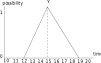
\psfig{file=./graphs/Y-time-point.eps}}
\vspace*{10pt}
\fcaption{\label{fig:fuzzy-validity-period}Transformation to obtain the FVP. The top graph shows the two triangular possibility distributions. The middle graph shows the convex hull validity period, the bottom one shows the result of the second transformation, which maintains the imprecision.}
%  \label{fig:fuzzy-validity-period}
\vspace*{13pt}

\begin{definition}
A \textbf{Possibilistic Valid-time Period} (\emph{PVP}) is an ill-known interval in time specifying when the data regarding an object is valid.
\end{definition}
A PVP is an ill-known interval in the sense of definition \ref{def;possibilistic-variable}, section \ref{subsec:possibilistic-variables}. Note that this representation is \emph{disjunctive}: the PVP represents only one crisp time interval, but that for some reason it is (partially) unknown.

The ill-known interval approach has many advantages from the representation by the FVP as demonstrated in \cite{Pons2011},\cite{Pons2012}. Table \ref{tbl:comparative-pvp-fvp} is a comparative between PVP and FVP. The following list defines the items in the comparative:

\begin{enumerate}
\item Domain: The domain of the possibility distribution modelled by the approach.
\item Implementation of relationships: How to implement a relationship.
\item Allen's relations: Are the Allen's relations defined?
\item Storage: The way the data is stored in the database.
\item Possibility measures: Does the framework provides always a possibility measure for any relation between the temporal elements?
\item Necessity measures:  Does the framework provides always a necessity measure for any relation between the temporal elements?
\end{enumerate}


%%
%% comparison table between pvp and fvp.
%%
\vglue13pt
%\begin{table}[htbp]
\tcap{Comparative PVP vs FVP}
%\centerline{\small DATA TYPES}
\vglue-6pt
\centerline{\small\baselineskip=13pt
\begin{tabular}{c p{2cm} p{2cm}}\\
Item & PVP & FVP\\
\hline
(1) & $\Pow(\R)$ & $\R$ \\
(2) & Ill-known constraints. & Ad-hoc operators. \\
(3) & $\checkmark$ & - \\
(4) & Two distributions one for each endpoint. & Only one distribution. \\ 
(5) & $\checkmark$ & $\checkmark$ \\
(6) & $\checkmark$ & - \\
\hline\\
\end{tabular}
\label{tbl:comparative-pvp-fvp}
} 

In the rest of the paper we will work only with PVP to represent valid-time intervals.


\subsection{\label{subsubsec:Understanding-valid-time-databases}Understanding Valid-time Databases}
This subsection is devoted to describe the behaviour of a crisp valid-time database. For the shake of simplicity, only the three main operations in the Data Manipulation Language \emph{DML} a.k.a \emph{CRUD} (CReate Update, Delete) operations are shown. Usually the DML operations in a temporal database are re-defined e.g. a typical update sentence in SQL could be re-defined by means of several insert and update sentences. Therefore, in order to be clear, these high level primitives in the DML for a valid-time database are usually noted as Insert, Modify and Delete. In the following subsections each primitive is defined and explained. Finally a illustrative example is given. For a more complete information on the behaviour of a bitemporal database, please refer to ~\cite{Jensen1994}.

\begin{definition}
Consider a relation $R$ in a temporal database, an entity $A$ given by the attributes $\left(a_1, \ldots, a_n \right)$ and the crisp time interval $I$ given by $\left[a,\ b\right] : a,b \in \T, a \leq b$. The pair $\left(A, I\right)$ expresses that the data regarding the entity A is valid during the crisp time interval I.  Note that the relation $R = \left(A, I \right) x \left(A, I \right)$. The following equation indicates that the pair $\left(A, I\right)$ is in the relation R:
\begin{equation}
\label{eq:rel-def}
\left( R, \left(A , I\right) \right)
\end{equation}
\end{definition}
\begin{example}
\label{ex:library-database}
 Consider a library database. Each physical book is stored with an identifier (ID), a title and the start and end loan dates respectively. Table \ref{tbl:library-sample} illustrates the first version of the database, after three insertions. In this example, $A = ($ ID, Title $)$ and $I = ($ Start Loan, End Loan $)$.
\end{example}





\vglue13pt
%\begin{table}[htbp]
\tcap{\label{tbl:library-sample}Sample library database}
\centerline{\small DATA TYPES}
\vglue-6pt
\centerline{\small\baselineskip=13pt
\begin{tabular}{c c c c}\\
\hline
\textbf{ID}  & Title  & Start Loan & End Loan \\
\hline
3 & Dracula & 15/3/2012 & 30/3/2012 \\
4 & Frankenstein & 25/3/2012 & 4/4/2012 \\
5 & Harry Potter & 18/3/2012 & 2/4/2012\\
3 & Dracula & 4/4/2012 & UC \\
\hline\\
\end{tabular}
}

In order to simplify the algorithms for the manipulation of data, some auxiliary functions and constants are defined:

\begin{definition}
 \label{def:until-changed}
\textbf{Until changed (UC):} To show that the data related to the entity $\left(A, I \right)$ is up-to-date, a special constant called \emph{Until Changed} is defined for the endpoint, $d$, of the time interval $I = \left(c, d\right)$. The value for this constant is considered to be $+\infty$. 
\end{definition}



If the pair $\left(A, I \right)$ with $I = \left(c, UC \right), c \in \T$ is in the relation $R$, then, it is said that the pair $\left(A, I \right)$ is \emph{current} in the relation.

For example, last row in Table \ref{tbl:library-sample}. The value for the time interval is $I = \left(4/4/2012 , UC \right)$. The meaning is that the book with ID = 3 was loaned the  4/4/2012 and it is still loaned. The book with ID = 3 is current in the relation.

\begin{definition}
\textbf{Current $\left(R, A \right)$:}
\label{def:current-in-relation}
This function returns a crisp time interval $I$ if the entity $A$ is current in the relation $R$ or the empty set, if the entity $A$ is not current in the relation.

%Consider an object $A$ and a relation $R$ in a temporal database. The function Current$\left(R, A \right)$ obtains the tuple $\left(A, I \right)$ that is current in the relation $R$, that is it, $I = \left[a, +\infty \right]$.

\begin{align}
\label{eq:current-in-relation}
\mbox{Current} \left(R, A \right) &=& \\ 
\begin{cases}
\nonumber
I & \mbox{ if } (A,I) \in R \wedge I = \left(c, UC \right), c \in \T\\
\emptyset & \mbox{ in any other case }
\end{cases}
\end{align}
\end{definition}

For example, the function Current(R, (3,`Dracula')) returns the time interval $I = \left(4/4/2012 , UC  \right)$. On the other hand, Current(R, (4,`Frankenstein')) returns the empty set.

The following two Allen's relations (see Figure \ref{fig:allen-rel}) are defined~\cite{Nagypal2003} to implement the auxiliary functions. 



\vspace*{13pt}
\begin{center}
{
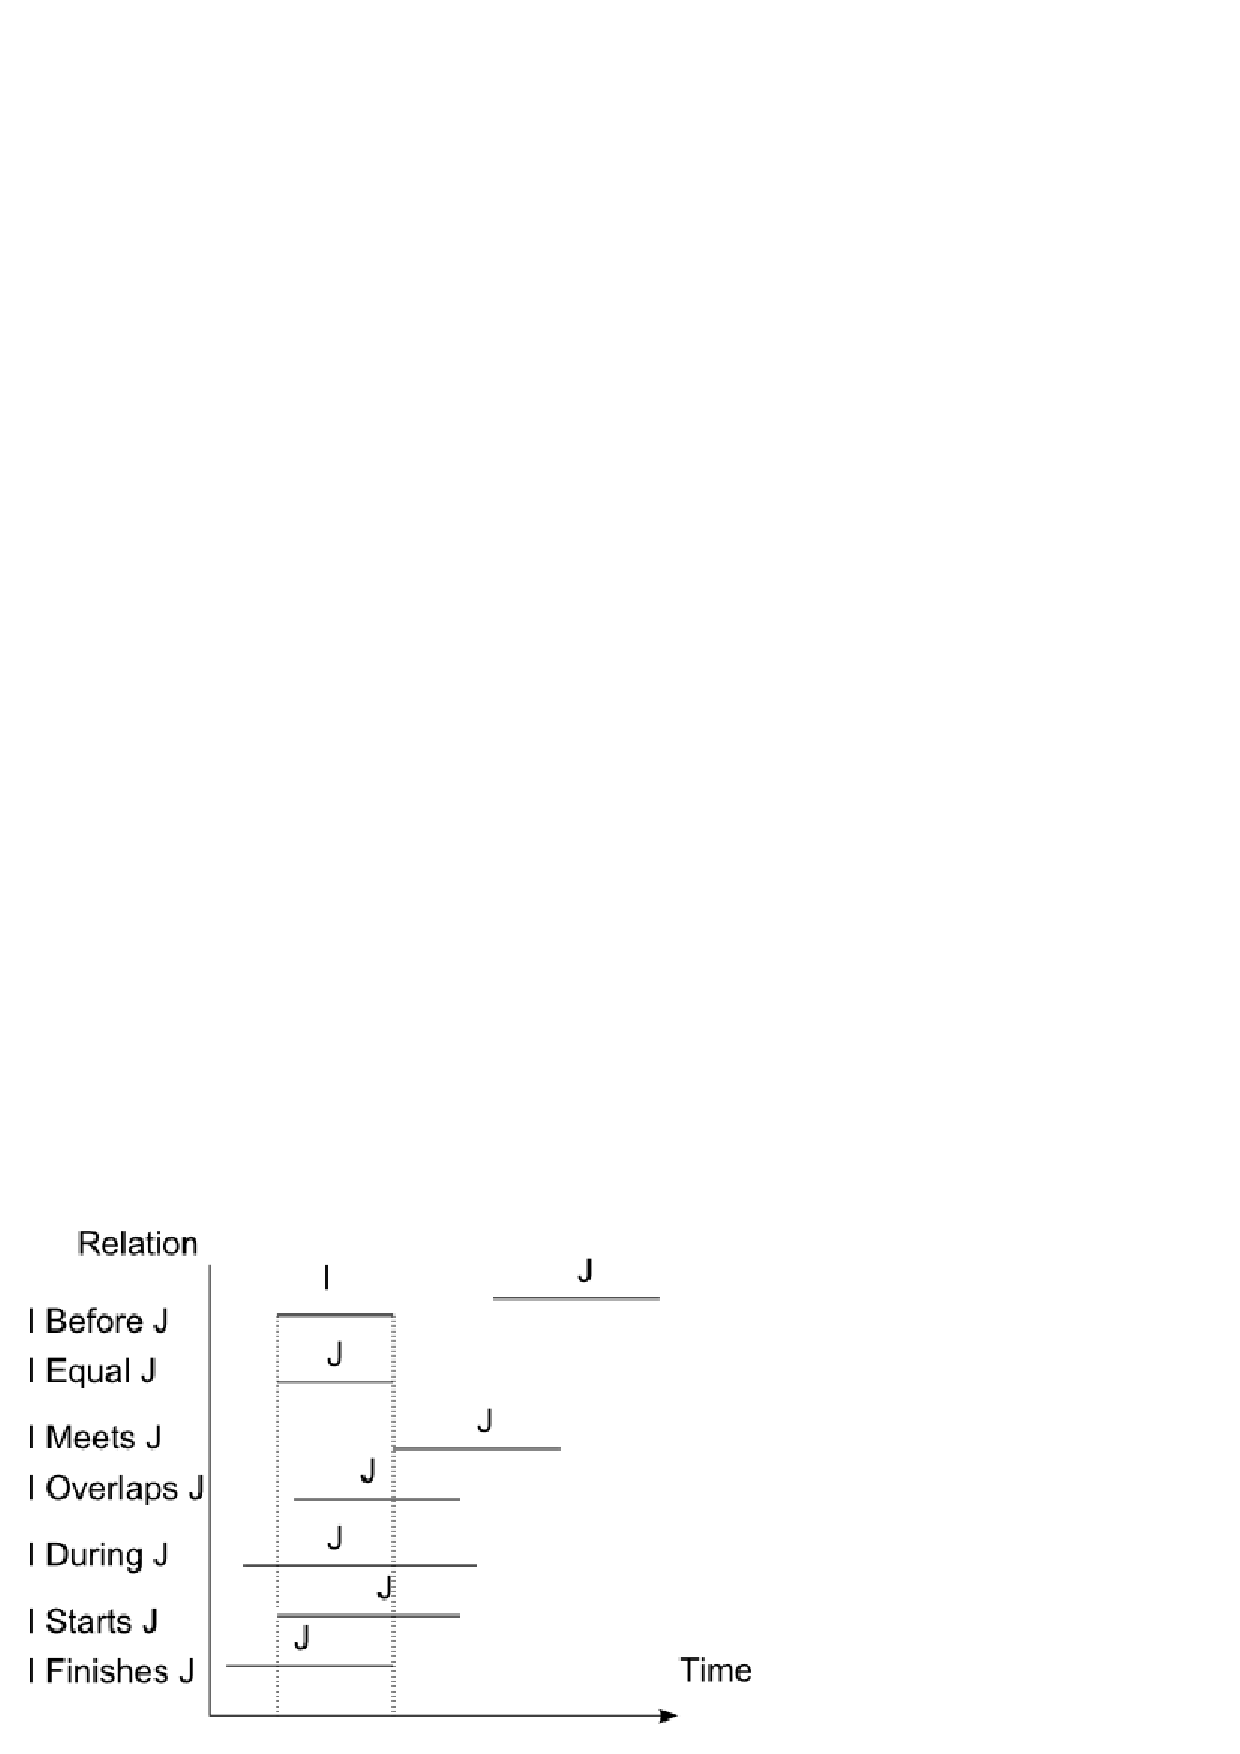
\includegraphics[scale=0.5]{./graphs/allen.pdf}

}
\end{center}
%\centerline{ 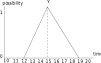
\psfig{file=./graphs/Y-time-point.eps}}
\vspace*{10pt}
\fcaption{\label{fig:allen-rel}Allen's relations for two crisp time intervals $I$ and $J$.}
\vspace*{13pt}


\begin{definition}
\textbf{Overlaps:}
 \label{def:overlaps}
Given two time intervals $I = \left(c, d \right)$ and $J = \left(e, f\right)$, it is said that I overlaps J if:
\begin{equation}
 \label{eqn:overlaps}
\text{I Overlaps J}  = \left(c > e  \right) \wedge \left(d < f  \right) 
\end{equation}
\end{definition}
  

\begin{definition}
\textbf{During:}
 \label{def:during}
Given two time intervals $I = \left(c, d \right)$ and $J = \left(e, f\right)$, it is said that I during J if:
\begin{equation}
 \label{eqn:during}
\text{I During J}  = \left(c < e  \right) \wedge \left(d > e  \right) \wedge \left(d < f \right)
\end{equation}
\end{definition}

\begin{definition}
\textbf{CloseR$\left( I, J \right)$:}
\label{def:close-a-crisp-interval-r}
Consider two crisp intervals $I= \left[c ,d \right]$ and $J= \left[e ,f \right]$. The CloseR$\left(I, J\right)$ function allows to close the right-open interval $I$ with respect to the first value $e$ in $J$:
\begin{align}
\label{eq:close-a-crisp-interval}
\mbox{CloseR} \left( I, J \right) &=& \\ 
\begin{cases}
\nonumber
%I & \mbox{ if } b \neq +\infty \\
%I=\left[a, c \right[ & \mbox{ if } b = +\infty \wedge J > I
\left[c, e \right[ & \mbox{ if } d = UC \wedge J \mbox{ During } I \\
I & \mbox{ in any other case.}
\end{cases}
\end{align}
\end{definition}

For example, consider two time intervals, $I = \left(4/4/2012, UC \right)$ and $J = \left(24/4/2012, UC \right)$. The result of applying the CloseR$\left(I, J \right)$ is $I = \left(4/4/2012, 23/4/2012 \right)$.




%Analogously, it is defined the function to close a left-open interval: 
%\begin{definition}
%\label{def:close-a-crisp-interval-l}
%CloseL$\left(I, J\right)$ 
%\begin{align}
%\mbox{CloseL} \left( I, J \right) &=& \\ 
%\begin{cases}
%\nonumber
%I & \mbox{ if } a \neq -\infty \\
%I=\left]d, b \right] & \mbox{ if } a = -\infty \wedge J < I
%\end{cases}
%\end{align}
%\end{definition}




%\begin{definition}
%\label{def:first-in-relation}
%Analogously, the function First$\left(R, A \right)$ obtains the tuple $\left(A, I \right)$ where $I$ is a right-open interval and which is the first version in the relation $R$, that is it, $I = \left[-\infty, b \right]$.
%\begin{align}
%\label{eq:first-in-relation}
%\mbox{First} \left(R, A \right) &=& \\ 
%\begin{cases}
%\nonumber
%I & \mbox{ if } \exists b \in I : (A,I) \in R \wedge a = -\infty \\
%\emptyset & \mbox{ in any other case }
%\end{cases}
%\end{align}
%
%\end{definition}



Now it is possible to close the current version of an entity by using \eqref{eq:close-a-crisp-interval} and \eqref{eq:current-in-relation}. This functionality is required to append new information about an existing entity in the relation.

\begin{definition}
\label{def:close-current-version}
Consider an entity $A$, the relation $R$ and a time interval $J$. Then, the function close-current$\left(R,\left(A,J\right) \right)$ closes any current version of the object $A$ if it exists and add the new version $\left(A, J \right)$.

\begin{eqnarray}
\label{eq:close-current}
\text{Close-current} \left(R, \left(A, J\right) \right) =\\
\begin{cases}
\nonumber
R - \left(A, I \right) \cup \left \lbrace \left(A, \mbox{ CloseR } \left(I, J\right) \right)\right \rbrace \cup \left \lbrace\left(A, J\right) \right \rbrace  \\
\nonumber
\mbox{ if } I = \mbox{ Current } \left(R, A \right)\\ %\wedge J > \mbox{ CloseR } \left(I, J \right)   \\
\nonumber R , \text{ in any other case}
\end{cases}
\end{eqnarray}
\end{definition}

For example, consider the book with ID = 3 in Table \ref{tbl:library-sample}. The current version was loaned on 4/4/2012. The book was returned to the library but, for some reason, the end loan date was not registered. The book is loaned again on 24/4/2012. Then, the Close-current function allows to close the current version of the book and insert a new version. First, the function CloseR is applied with $I = \left(4/4/2012, UC \right)$ and $J = \left(24/4/2012, UC \right)$. Hence, the value for the time interval $I$ is $ \left(4/4/2012, 23/4/2012 \right)$. Then, the modifications on the value for the time interval $I$ are stored. Finally, a new row with the current values of the book and the time interval $J$ is stored.
The result of this operation is illustrated on Table \ref{tbl:library-sample-2}.




%It is also possible to append at the beggining by using \eqref{def:close-a-crisp-interval-l} and \eqref{def:first-in-relation}.
%\begin{definition}
%\label{def:append-first-version}
%Consider an object $A$, the relation $R$ and a time interval $J$. Then, the function append-first$\left(R,A,J \right)$ closes any right open version of the object $A$ if it exists and add the new version $\left(A, J \right)$.
%
%\begin{eqnarray}
%%\label{eq:close-current}
%\text{Append-first} \left(R, A, J \right) =\\
%\begin{cases}
%\nonumber
%\big \lbrace R - \left(A, I \right) \cup \left \lbrace \left(A, \mbox{ CloseL } \left(I, J\right) \right) \cup \left(A, J\right)\right \rbrace  \big \rbrace \\
%\nonumber
%\mbox{ if } I = \mbox{ First } \left(R, A \right) \wedge J < \mbox{ CloseL } \left(I, J \right)   \\
%\nonumber R , \text{ in any other case}
%\end{cases}
%\end{eqnarray}
%\end{definition}
\subsubsection{\label{subsubsec:modify}Modify}
This operation adds new information about an existing entity $A$ in the relation $R$. The modify operation does not remove any previous value of the object $A$. It closes the current version for the entity $A$ and adds a new version.


%Note that the modify operation is only applicable when the object $A$ is current in the relation $R$; $ \left(A, I \right) \in R, I = \left[a, +\infty \right]$.

\begin{align}
\label{eq:modify}
\MOD \left( R, \left(A, I \right)\right) =\\
%\begin{cases}
\nonumber
\mbox{ Close-current }\left(R, \left(A, I\right) \right) %\\
% \mbox{ if Current}\left(R ,A \right) \neq \emptyset \\
% R,  \mbox{ otherwise }
%\end{cases}
\end{align}


\subsubsection{\label{subsubsec:insert}Insert}
The user wants to store an object $A$ which is valid in the relation $R$ during the time interval specified by $I = \left(a, b \right)$.
%
%
%The interpretation of the insert operation is the following: The user wants to store in the database that an object $A$  is true for some period(s) of time $I$ in the given relation $R$. To indicate that the object $A$ is current in the relation, the special value Until Current, $\UC$  is used. 
There are two main cases when performing a create operation:
\begin{enumerate}
\item The object $A$ was never in the relation $R$: The object is added with the valid-time indicated by the crisp interval $I$. In the example, this correspond with the following insertion sentences:
\begin{verbatim}
Insert(3,'Dracula',
(15/3/2012, 30/3/2012));
Insert(4,'Frankenstein',
(25/3/2012, 4/4/2012));
Insert(5,'Harry Potter',
(18/3/2012, 2/4/2012));
\end{verbatim}


\item The object $A$ is in the relation $R$. Depending on the value of the time interval $I$, there are three possibilities:
	\begin{enumerate}
	\item Insert $\left(A, I\right)$ in the relation $R$. If the time interval $I$ does not overlap any other valid-time interval in the relation $R$. For example, consider that the book with ID 3 is loaned on 4/4/2012 but the book has not been returned yet. This is illustrated in Table \ref{tbl:library-sample}. The insert sentence is:
	      \begin{verbatim}
Insert(3,'Dracula',
(4/4/2012, UC));
	      \end{verbatim}


	\item Modify and close the current version of $A$ and insert $\left(A, I\right)$. For example, consider now that the book with ID 3 is loaned  the 24/4/2012. Here the problem is that the book with ID 3 was loaned on 4/4/2012, but not returned. If the book is already in the library for a new loan, then it is necessary to set the return date and add a new row with the new loan date. This is illustrated in Table \ref{tbl:library-sample-2}, the insert sentence is:
	    \begin{verbatim}
Insert(3,'Dracula',
(24/4/2012, UC));
	      \end{verbatim}
	\item Reject the insertion, if the time interval $I$ does overlap any existing valid-time interval for the object $A$ in the relation $R$. For example, consider now that the librarian wants to introduce a past loan for the book with ID 3. The book was loaned on 6/4/12/2012 and returned on 25/4/2012. As this interval does overlaps other time intervals, it is not possible that the book was loaned in that time interval.Therefore, the insertion is rejected. The insert sentence is:

	      \begin{verbatim}
Insert(3,'Dracula',
(6/4/12/2012,25/4/2012));
	    \end{verbatim}


	\end{enumerate}

\end{enumerate}

\vglue13pt
%\begin{table}[htbp]
\tcap{\label{tbl:library-sample-2}Sample library database}
%\centerline{\small DATA TYPES}
\vglue-6pt
\centerline{\small\baselineskip=13pt
\begin{tabular}{c c c c}\\
\hline
\textbf{ID}  & Title  & Start Loan & End Loan \\
\hline
3 & Dracula & 15/3/2012 & 30/3/2012 \\
4 & Frankenstein & 25/3/2012 & 4/4/2012 \\
5 & Harry Potter & 18/3/2012 & 2/4/2012\\
3 & Dracula & 4/4/2012 & 23/4/2012 \\
3 & Dracula & 24/4/2012 & UC \\
\hline\\
\end{tabular}
}



The algorithm for the implementation of the insert operation is the following:

\begin{align}
\label{eq:insert}
\INS \left(R ,\left(A, I\right)\right) =\\
\begin{cases}
\nonumber
R \cup \left(A, I \right) & \mbox{ if }  (A, I ) \not \in R  \vee \\
 &   \left(A, J\right) \in R \wedge \lnot \left(I \mbox{ Overlaps } J\right) \\
\mbox{modify(R,(A,I))} & \mbox{ otherwise }    %\mbox{ if } \exists J \left(A,J\right) \in R \wedge \mbox{Current(A,J)} \\ 
%R, &   
\end{cases} 	
\end{align}

\subsubsection{\label{subsubsec:del}Delete}
The delete operation logically removes a current entity $A$ which is valid in the relation $R$:
\begin{align}
\label{eq:delete}
\DEL \left(R ,A \right) =\\
\begin{cases}
\nonumber
R - \left(A, I \right), & \forall \left( A, I \right) \in R\\
R, & \mbox{ otherwise }  
\end{cases} 	
\end{align}

For example, consider that the librarian wants to delete the history for the book with ID = 3. The result of this operation is shown in Table \ref{tbl:library-sample-3}. The delete sentence is:

\begin{verbatim}
 Delete(3,'Dracula');
\end{verbatim}


\vglue13pt
%\begin{table}[htbp]
\tcap{\label{tbl:library-sample-3}Sample library database}
%\centerline{\small DATA TYPES}
\vglue-6pt
\centerline{\small\baselineskip=13pt
\begin{tabular}{c c c c}\\
\hline
\textbf{ID}  & Title  & Start Loan & End Loan \\
\hline
4 & Frankenstein & 25/3/2012 & 4/4/2012 \\
5 & Harry Potter IV & 18/3/2012 & 2/4/2012\\
\hline\\
\end{tabular}
}


\subsubsection{\label{subsubsec:revise}Revise}
This operation replaces the old values for the entity $A'= \left(a_1', \ldots, a_n' \right) $ with the new values specified by $A = \left(a_1, \ldots, a_n \right)$ in the relation $R$, at a given time interval $I$. This operation is used when a correction on the values for the entity $A$ should be done.
\begin{align}
\REV\left(R, \left(A, I \right) \right)=\\
\begin{cases}
\nonumber
 R - \left(A', I \right) \cup \left \lbrace \left(A, I \right) \right \rbrace & \mbox{ if } \left(A', I \right) \in R  \\
   %: A = \left(a_1, \ldots, a_n \right),\\
%A'= \left(a_1', \ldots, a_n' \right)   \\   
R & \mbox{ otherwise }
\end{cases}
\end{align} 

For example, consider now that the librarian wants to make a correction in the title for the book with ID = 5. The new title is `Harry Potter IV'. The result of this operation is illustrated in Table \ref{tbl:library-sample-3}.
 Then, the revise sentence is:

\begin{verbatim}
Revise(5,'Harry Potter IV', 
(18/3/2012, 2/4/2012));
\end{verbatim}

